



\documentclass{beamer}
\usepackage{multimedia}
\usepackage{graphicx}
\usetheme{Madrid}

\usepackage{amsmath,amssymb}
\usepackage{bm}
\usepackage[absolute,overlay]{textpos}
\usepackage{mathtools}
\usepackage{courier}
\usepackage{tikz}
\usepackage{lmodern}
\beamertemplatenavigationsymbolsempty
\usefonttheme[onlymath]{serif}
\graphicspath{{./gfx/}}

\newcommand{\ppos}{q}
\newcommand{\pvel}{u}
\newcommand{\fpos}{r}
\newcommand{\fvel}{v}
\newcommand{\corr}{\text{corr}}
\newcommand{\dpr}{\text{\tiny DP}}
\newcommand{\qtd}{\text{\tiny q2D}}
\renewcommand{\vec}[1]{\bm{#1}}
\newcommand{\tens}[1]{\bm{\mathcal{#1}}}
\newcommand{\oper}[1]{\mathcal{#1}}
\newcommand{\uammd}{\gls{UAMMD}\xspace}
\newcommand{\gpu}{\gls{GPU}\xspace}
\newcommand{\dt}{\delta t}
\newcommand{\kT}{k_B T}
\newcommand{\sinc}{\textrm{sinc}}
\newcommand{\floor}{\textrm{floor}}
\newcommand{\near}{\textrm{near}}
\newcommand{\far}{\textrm{far}}
\newcommand{\half}{\frac{1}{2}}
\newcommand{\red}[1]{{\color{red}#1}}
\newcommand{\fou}[1]{\widehat{#1}}
\newcommand{\noise}{\widetilde{W}}

\newcommand{\executeiffilenewer}[3]{
  \ifnum
  \pdfstrcmp{\pdffilemoddate{#1}}{\pdffilemoddate{#2}}>0
  {\immediate\write18{#3}}
  \fi
}
\newcommand{\includesvg}[2][width=\columnwidth]{
  \executeiffilenewer{#2.svg}{#2.pdf}
  {inkscape -D #2.svg --export-type=pdf } %  --export-latex}
  %\def\svgwidth{#2}
  % \input{#1.pdf_tex}
  \includegraphics[#1]{#2.pdf}
}




\title{Complex fluids in the GPU era}
\subtitle{Algorithms and simulations}
\author{Raul P. Pelaez}

\institute{Universidad Autónoma de Madrid}
\date{\today}


\begin{document}


\begin{frame}
  \titlepage
\end{frame}

\begin{frame}
  \tableofcontents
\end{frame}




\section{Contents}
\begin{frame}
  \frametitle{\insertsection}
  \begin{itemize}
  \item UAMMD's functionalities
  \item Particle-based and grid based
  \item Code structure
    \begin{itemize}
    \item open-source
    \item adaptable
    \item ...
    \end{itemize}
  \end{itemize}
\end{frame}

\section{Complex fluids}
\begin{frame}
  \frametitle{Complex fluids}
  \framesubtitle{Usual levels of coarse-grained description}
  \begin{columns}
    \begin{column}{0.5\linewidth}
      \begin{tikzpicture}
        \node[anchor=south west,inner sep=0] (image) at (0,0) {
          \begin{tikzpicture}
            \node[anchor = south west, inner sep = 0] (image) {\includesvg[width=1.05\linewidth]{gfx/multiscale}};
            \begin{scope}[shift={(image.south west)},x={(image.south east)},y={(image.north west)}]
              % Draw a overlaying grid to easily see where the rectangles must be, this can be commented out in the final version
              % \draw foreach \xy in {0,0.1,...,1.001}{
              % (\xy,0) -- node[pos=0,below]{\pgfmathprintnumber{\xy}} (\xy,1)
              % (0,\xy) -- node[pos=0,left]{\pgfmathprintnumber{\xy}} (1,\xy)};
              \foreach[count=\i] \mypath in {
                {(0,1) rectangle (0.48,0.55)},
                {(0,0.55) rectangle (0.48,0)},
                {(0.48,1) rectangle (1.0,0.55)},
                {(0.48,0.55) rectangle (1,0)},
                {(0,1) rectangle (1,0)}
              }{
                \filldraw<\i>[white,opacity=0.9,even odd rule] (0,0) rectangle (1,1) \mypath;
                \draw<\i>[white, thick] \mypath;
              }
            \end{scope}
          \end{tikzpicture}
        };
        \only<1-4>{\node[align=center] at (image.center) {
          \begin{minipage}{1.04\linewidth}
            \only<1,3>{\vspace*{50pt}}
            \only<2,4>{\vspace*{-100pt}}
            \only<3>{\vspace*{40pt}}
            \begin{block}{
                \only<1>{Molecular Dynamics (MD)}
                \only<2>{Langevin Dynamics (LD)}
                \only<3>{Immersed Boundary Method (IBM)}
                \only<4>{Brownian Dynamics (BD)}
              }              
              \begin{equation*}
                \only<1>{
                  \begin{aligned}
                    m\ddot{\vec{\ppos}} &= \vec{F}\\
                    \vec{\pvel} &= \dot{\vec{\ppos}}
                  \end{aligned}
                }
                \only<2>{
                  m d\vec{\pvel} = \vec{F}dt - \xi\vec{\pvel}dt +  \sqrt{2\xi\kT}\vec{\noise}                 
                }
                \only<3>{
                  \begin{aligned}
                    &\rho\partial_t\vec{\fvel} = -\nabla\cdot \tens{\sigma} + \vec{f} + \text{fluct}\\[-5pt]
                    &\int_{V_p}\vec{f}d\vec{\fpos} = \vec{F}\\[-5pt]
                    &\vec{u} = \int_{V_p}\vec{\fvel}(\vec{\fpos}, t)d\vec{\fpos}
                  \end{aligned}
                }
                \only<4>{
                  \begin{aligned}
                    d\vec{\ppos} =& \tens{M}\vec{F}dt + \sqrt{2\kT\tens{M}}d\vec{\noise}\\
                    &+ \kT\vec{\partial}_{\vec{\ppos}}\cdot\tens{M}dt.
                  \end{aligned}
                }
              \end{equation*}
            \end{block}
          \end{minipage}          
        };}
      \end{tikzpicture}
    \end{column}
    \begin{column}{0.45\linewidth}
%      \only<1,3>{\vspace*{-100pt}}
%      \only<2,4>{\vspace*{100pt}}
      \begin{center}
        \textbf{Relevant variables:}
      \end{center}
      \begin{itemize}
      \item<1-> $\vec{q}_i$: Position of particle $i$.
      \item<1-> $\vec{u}_i$: Velocity of particle $i$.
      \item<2,5-> $\xi(\vec{q}_{ij})$: Friction kernel.
      \item<3,5-> $\vec{v}(\vec{r},t)$: Fluid velocity field.
      \item<4-> $M(\vec{q}_{ij})$: Mobility tensor.
      \end{itemize}
    \end{column}
  \end{columns}
  \only<6>{
    \begin{textblock*}{100mm}(12mm,0.5\textheight)
    \begin{alertblock}{Its always}
      Interacting ``particles'' with a state that ``evolves'' in time.
    \end{alertblock}
    \end{textblock*}
  }
\end{frame}

\section{UAMMD's functionalities}
\begin{frame}
  \frametitle{Universally Adaptable Multiscale Molecular Dynamics}
  \framesubtitle{Functionalities}
  \begin{columns}
    \begin{column}{0.5\linewidth}
      \begin{itemize}
      \item a
      \item b
      \end{itemize}
    \end{column}
    \begin{column}{0.5\linewidth}
      \begin{figure}
        \centering
        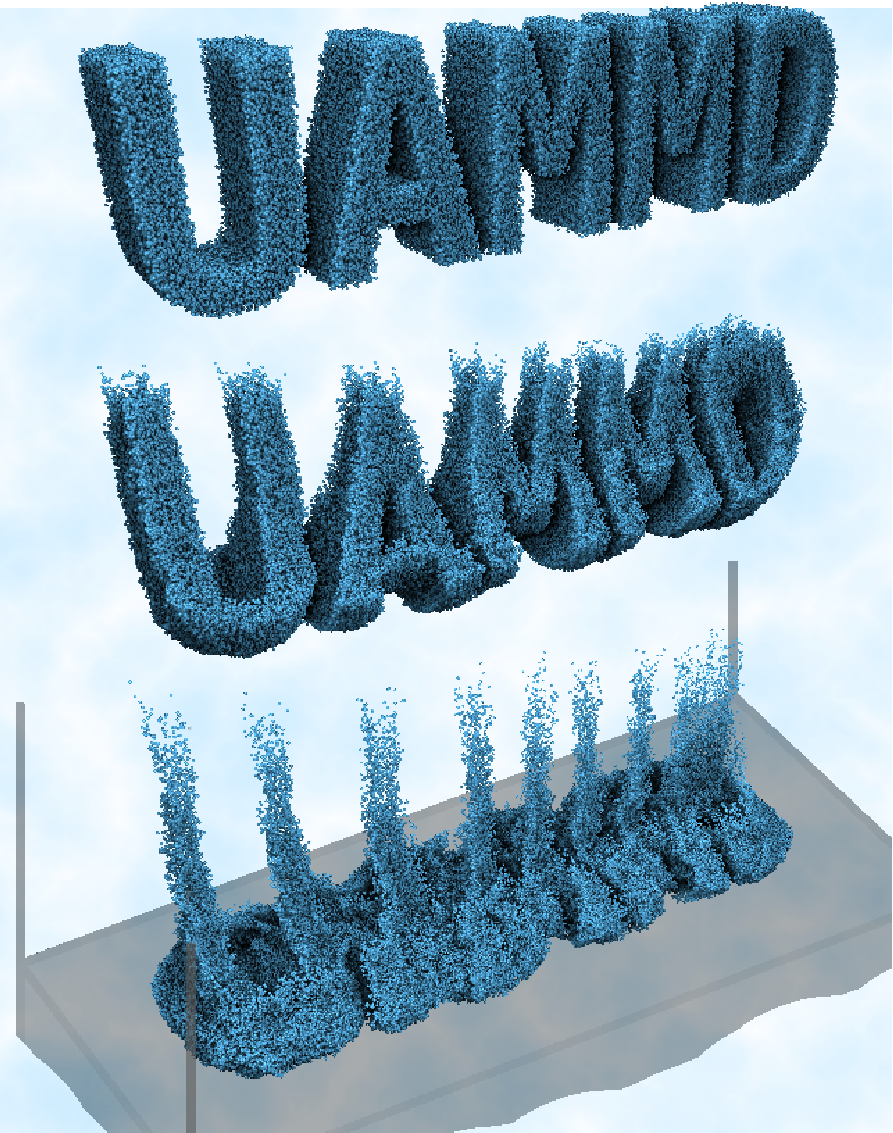
\includegraphics[height=0.75\textheight]{poster.png}
      \end{figure}
    \end{column}
  \end{columns}
\end{frame}


\section{Introduction}
\begin{frame}
  \frametitle{\insertsection}
  \begin{itemize}
  \item Outline
  \item Physics, algorithms and implementation
  \item This thesis contributions
  \end{itemize}
\end{frame}

\subsection{Complex fluids}
\begin{frame}
  \frametitle{\insertsubsectionnavigation{\linewidth}}
  \begin{itemize}
  \item What a complex fluid is and why we care
  \item Coarse-graining
  \end{itemize}
\end{frame}
\subsubsection{A typical system of interest}
\begin{frame}
  \frametitle{\insertsubsectionnavigation{\linewidth}} 
  \framesubtitle{\insertsubsubsection}
  \begin{itemize}
  \item ``We want to study this particular system (a virus?, QCM?)''
  \item Problems that arise when trying to simulate this system
  \item The message is: We need new theory and algorithms. If we carefully design a software for a system like this, we end up with something that is also valid for things like MD,  SPH, DPD,...
  \end{itemize}
\end{frame}
\subsection{High performance computing in complex fluids}
\begin{frame}
  \frametitle{\insertsubsectionnavigation{\linewidth}} 
  \begin{itemize}
  \item The GPU
  \item Other software packages
  \item Trying to keep it simple
  \end{itemize}
\end{frame}


\section{The different ingredients of a complex fluid simulation}

\begin{frame}
  \frametitle{\insertsectionnavigation{\linewidth}} 
  \begin{itemize}
  \item Hydrodynamics
  \item Particle interactions
  \item Electrostatics
  \end{itemize}
\end{frame}

\subsection{Hydrodynamics}
\begin{frame}
  \frametitle{\insertsubsectionnavigation{\linewidth}}
  \begin{itemize}
  \item Fluid dynamics
  \item Particle-fluid coupling (IBM)
  \item Pseudo-spectral solvers (FCM)
  \end{itemize}
\end{frame}

\subsection{Particle interactions}
\begin{frame}
  \frametitle{\insertsubsectionnavigation{\linewidth}}
  \begin{itemize}
  \item Neighbour lists
  \item bonds
  \end{itemize}
\end{frame}

\subsection{Electrostatics}
\begin{frame}
  \frametitle{\insertsubsectionnavigation{\linewidth}}
  \begin{itemize}
  \item Poisson equation
  \item Reuse of FCM
  \end{itemize}  
\end{frame}
    
\subsection{UAMMD: A GPU framework for complex fluids}
\begin{frame}
  \frametitle{\insertsubsectionnavigation{\linewidth}} 
  \begin{itemize}
  \item What UAMMD is and tries to achieve
  \item ``UAMMD has enabled the community to study hydrodynamics in new systems''
  \item Not trying to sell UAMMD, just showcase what it can do.    
  \end{itemize}
\end{frame}

\section{New physics}

\begin{frame}
  \frametitle{\insertsectionnavigation{\linewidth}} 
  \begin{itemize}
  \item List works using UAMMD, what level of detail here?
  \end{itemize}
\end{frame}

\end{document}